\subsection{DFA accepting a binary substring divisible by prime number}

\renewcommand{\CURPATH}{synth/DFA}

A problem: construct a regular expression accepting binary number divisible by 3.

"1111011" (123) is, "101010101011" (2731) is not.

Some discussion and the correct expressions:

\begin{itemize}
\item \url{https://stackoverflow.com/questions/7974655/regex-for-binary-multiple-of-3}
\item \url{https://stackoverflow.com/questions/844867/check-if-a-number-is-divisible-by-3}
\item \url{https://stackoverflow.com/questions/867279/regular-expression-to-define-some-binary-sequence}
\item \url{https://www.regextester.com/96234}
\end{itemize}

I couldn't generate \ac{RE}, but I can generate a minimal \ac{DFA}:

\lstinputlisting[style=custompy]{\CURPATH/2.py}

As you can see, it has testing procedure, which is, in turn, can be used instead of RE matcher, if you really need to match
numbers divisible by 3.

tates in double circles --- initial (\verb|S_0|) and accepting:

\begin{figure}[H]
\centering
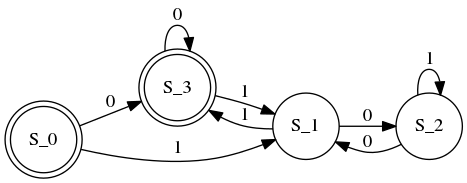
\includegraphics[scale=0.7]{\CURPATH/2_3.png}
\caption{DFA for numbers divisible by 3}
\end{figure}

... is almost like the one someone posted \href{https://stackoverflow.com/questions/7974655/regex-for-binary-multiple-of-3}{here},
but my solution has two separate states as initial and accepting.

\begin{figure}[H]
\centering
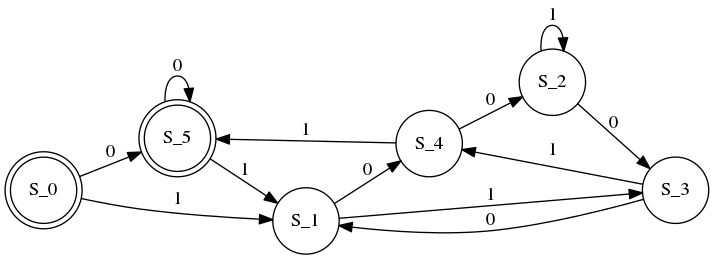
\includegraphics[scale=0.7]{\CURPATH/2_5.png}
\caption{DFA for numbers divisible by 5}
\end{figure}

\begin{figure}[H]
\centering
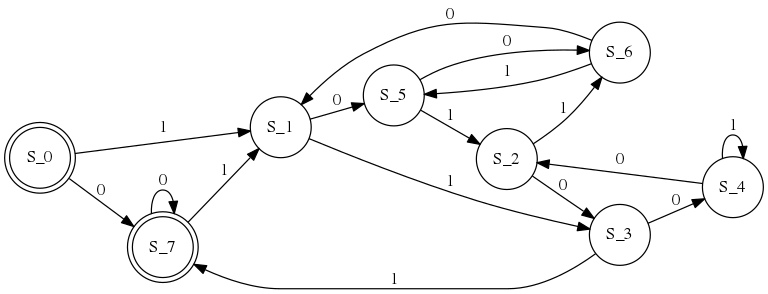
\includegraphics[scale=0.7]{\CURPATH/2_7.png}
\caption{DFA for numbers divisible by 7}
\end{figure}

\begin{figure}[H]
\centering
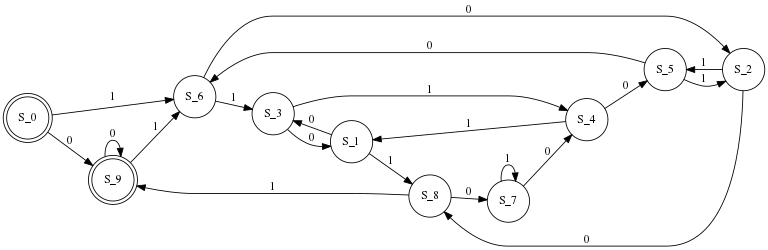
\includegraphics[scale=0.7]{\CURPATH/2_9.png}
\caption{DFA for numbers divisible by 9. Probably not an easy thing to find it manually}
\end{figure}

\begin{figure}[H]
\centering
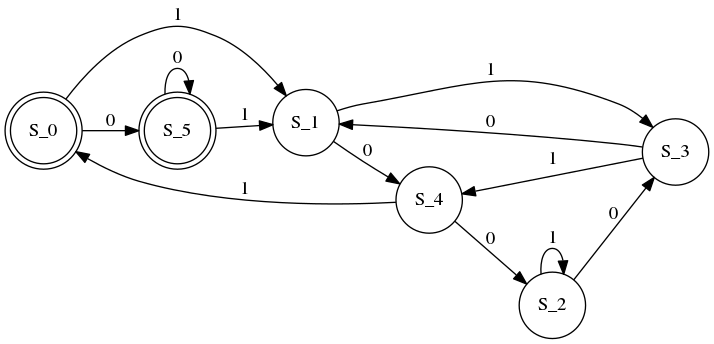
\includegraphics[scale=0.7]{\CURPATH/2_10.png}
\caption{DFA for numbers divisible by 10. Not a prime, so the DFA is smaller}
\end{figure}

These DFAs are guaranteed to be minimal.
Further work: convert them to \ac{RE}...

